\subsection{Build} \label{sec:build}

The build of software products is usually done on build servers without manual
interaction. In the Eclipse ecosystem several build systems are available. The
one gaining most attention nowadays is Maven Tycho, which is a set of plugins
for the well-known Maven build framework.

In Maven, the build descriptors are so-called POM files (usually \texttt{pom.xml}). For
the LWC example we have added such POM files to enable a headless build.

\subsubsection{settings.xml}
Maven needs to know about repositories from where it can download artifacts. By
default, Maven only knows about Maven Central, which is the repository hosted by
Apache. For our build we need to consume some artifacts that are not available
at Maven Central:
\begin{itemize} 
\item The Fornax Workflow plugin is used to execute MWE workflows to
generate code from the Xtext grammar.
\item The Xtend plugin compiles Xtend classes to Java code.
\end{itemize} 

All plugin dependencies must be resolvable through Eclipse p2 repositories. The
layout p2 is a special layout contributed by Tycho. The plugins consume
dependencies from
\begin{itemize}
  \item Eclipse Juno: Composite repository of the Eclipse Juno simultaneous
  release. Most plugins are resolved through this repository.
  \item Eclipse Orbit: Orbit contains OSGi bundles of 3rd party components
  (like logj, javax.faces, javax.inject, Google Guava etc.).
  \item Eclipse Xtext: The release repository for Xtext, Xtend, MWE2.
\end{itemize} 

In \texttt{settings.xml}, repository configurations must be contained in a profile. We
define a profile \texttt{external-repositories}, which is activated by default
in the \texttt{activeProfiles} section.

\begin{lstlisting}[language=XML]
<settings>
  <activeProfiles>
    <activeProfile>external-repositories</activeProfile>
  </activeProfiles>
  <profiles>
    <profile>
      <id>external-repositories</id>
      <repositories>
        <repository>
          <id>Eclipse Juno</id>
          <layout>p2</layout>
          <url>http://download.eclipse.org/releases/juno</url>
        </repository>
        <repository>
          <id>Eclipse Orbit</id>
          <layout>p2</layout>
          <url>http://download.eclipse.org/tools/orbit/downloads/drops/R20120526062928/repository/
          </url>
        </repository>
        <repository>
          <id>Eclipse Xtext</id>
          <layout>p2</layout>
          <url>http://download.eclipse.org/modeling/tmf/xtext/updates/composite/releases/
          </url>
        </repository>
      </repositories>
      <pluginRepositories>
        <pluginRepository>
          <id>fornax.releases</id>
          <name>Fornax Release Repository</name>
          <url>http://www.fornax-platform.org/nexus/content/repositories/releases/
          </url>
        </pluginRepository>
        <pluginRepository>
          <id>xtend</id>
          <url>http://build.eclipse.org/common/xtend/maven/</url>
        </pluginRepository>
      </pluginRepositories>
    </profile>
  </profiles>
</settings>
\end{lstlisting}

The settings file is placed in the repository under
/devenv/lwc13.devenv/settings.xml.

In order to use this settings file, it has to be put to <HOME>/.m2 or passed
with the ``-s'' option to the \texttt{mvn} command.

\subsubsection{Parent POM}
Since Maven supports a simple POM inheritance, it is common to extract common
settings for a set of project modules into a so-called Parent POM. This pom.xml
fil is placed in the root of the
repository\footnote{\url{http://code.google.com/a/eclipselabs.org/p/lwc13-xtext/source/browse/pom.xml}}.

The parent POM is responsible for different things:
\begin{itemize}
\item Definition of the common groupId and version
\begin{lstlisting}[language=XML]
  <groupId>org.eclipse.xtext.example.ql</groupId>
  <version>1.0.0-SNAPSHOT</version>
\end{lstlisting}
\item Tycho Plugin configuration. Note the
\texttt{<extensions>true</extensions>} entry. To make the Tycho version that is
used easier configurable, a property \texttt{tycho-version} is defined, which is used for
all Tycho plugin configurations.
\begin{lstlisting}[language=XML]
  <properties>
    <tycho-version>0.17.0</tycho-version>
  </properties>
  <build>
    <plugins>
      <plugin>
        <groupId>org.eclipse.tycho</groupId>
        <artifactId>tycho-maven-plugin</artifactId>
        <version>${tycho-version}</version>
        <extensions>true</extensions>
      </plugin>
      ...
\end{lstlisting}
\item Supported Target Environments. Eclipse is partially OS dependent. Which
platforms should be considered in the target platform configuration is
configured with the target-platform-configuration plugin.
\begin{lstlisting}[language=XML]
  <plugin>
    <groupId>org.eclipse.tycho</groupId>
    <artifactId>target-platform-configuration</artifactId>
    <version>${tycho-version}</version>
    <configuration>
      <resolver>p2</resolver>
      <pomDependencies>consider</pomDependencies>
      <environments>
        <environment>
          <os>win32</os>
          <ws>win32</ws>
          <arch>x86</arch>
        </environment>
        <environment>
          <os>win32</os>
          <ws>win32</ws>
          <arch>x86_64</arch>
        </environment>
        <environment>
          <os>macosx</os>
          <ws>cocoa</ws>
          <arch>x86_64</arch>
        </environment>
      </environments>
    </configuration>
  </plugin>
\end{lstlisting}
\item Java Source Code version. The produced code requires Java 1.6 for
compilation. This needs to be configured at the \texttt{tycho-compiler-plugin}.
\begin{lstlisting}[language=XML]
  <plugin>
    <groupId>org.eclipse.tycho</groupId>
    <artifactId>tycho-compiler-plugin</artifactId>
    <version>${tycho-version}</version>
    <configuration>
      <encoding>UTF-8</encoding>
      <meminitial>128m</meminitial>
      <maxmem>1024m</maxmem>
      <source>6.0</source>
      <target>6.0</target>
      <verbose>true</verbose>
    </configuration>
  </plugin>
\end{lstlisting}
\item Maven Plugin Management. In the \texttt{pluginManagement} section the plugins that
potentially participate in the build are configured with their versions. This is
because Maven would select the latest available version of a plugin instead and
prints warnings during the build. It is better to fix the versions of plugins
that are used to those with which the build has been tested. Also basic plugin
configurations can be added here.
\begin{lstlisting}[language=XML]
  <plugin>
    <groupId>org.eclipse.tycho</groupId>
    <artifactId>tycho-p2-repository-plugin</artifactId>
    <version>${tycho-version}</version>
  </plugin>
  <plugin>
    <groupId>org.apache.maven.plugins</groupId>
    <artifactId>maven-clean-plugin</artifactId>
    <version>2.4.1</version>
  </plugin>
  ...
\end{lstlisting}
\end{itemize}

\subsubsection{Reactor POM}
The project consists of several modules, which is called a
\href{http://www.sonatype.com/books/mvnex-book/reference/multimodule.html}{Multi
Module Project} in Maven terms. The modules of a project are listed in a
\texttt{<modules>} section. Often the modules are enlisted in the Parent POM,
but we splitted this. There is a POM that only contains module entries in the
\texttt{projects}
folder\footnote{\url{http://code.google.com/a/eclipselabs.org/p/lwc13-xtext/source/browse/projects/pom.xml}}:

\begin{lstlisting}[language=XML]
  <modules>
    <module>org.eclipse.xtext.example.ql</module>
    <module>org.eclipse.xtext.example.ql.ui</module>
    <module>org.eclipse.xtext.example.qls</module>
    <module>org.eclipse.xtext.example.qls.ui</module>
    <module>org.eclipse.xtext.example.ql.sdk</module>
    <module>org.eclipse.xtext.example.ql.repository</module>
  </modules>
\end{lstlisting}

When building the DSL projects, this POM has to be executed. Assuming the build
is executed from the repository root, the typical build command would be:

\begin{lstlisting}
mvn -s devenv/lwc13.devenv/settings.xml -f projects/pom.xml clean install
\end{lstlisting}

\subsubsection{QL Runtime Project POM}
Let's look a bit at the POM of the QL Runtime Project
org.eclipse.xtext.example.ql.

\begin{lstlisting}[language=XML]
<?xml version="1.0" encoding="UTF-8"?>
<project xsi:schemaLocation="http://maven.apache.org/POM/4.0.0 http://maven.apache.org/xsd/maven-4.0.0.xsd" xmlns="http://maven.apache.org/POM/4.0.0"
  xmlns:xsi="http://www.w3.org/2001/XMLSchema-instance">
  <modelVersion>4.0.0</modelVersion>
  <parent>
    <groupId>org.eclipse.xtext.example.ql</groupId>
    <artifactId>parent</artifactId>
    <version>1.0.0-SNAPSHOT</version>
    <relativePath>../../pom.xml</relativePath>
  </parent>
  <artifactId>org.eclipse.xtext.example.ql</artifactId>
  ...
\end{lstlisting}

At the beginning we have the typical Maven coordinates and parent dependency.
The Parent POM is at the root of the repository, which is 2 directories up. The
POM one directory up is the Reactor POM. Note that it is important to mention
here the exact same version as declared in the Parent POM. This module inherits
the parent's version and groupId coordinates, only the artifactId changes.

Maven Tycho enforces that the POM version matches \texttt{Bundle-Version}, and
the \texttt{artifactId} must be equal to the \texttt{Bundle-SymbolicName} of the manifest. A bit
special are SNAPSHOT versions, which is a special Maven concept for intermediate
development versions of artifacts. When the project version is a snapshot
version, the bundle version must have an additional qualifier. In our case here,
the project version is \texttt{1.0.0-SNAPSHOT}, which means the bundle version must be
\texttt{1.0.0.qualifier}. The qualifier gets replaced at build time by a timestamp.

\begin{lstlisting}
Bundle-Name: org.eclipse.xtext.example.ql
Bundle-Version: 1.0.0.qualifier
\end{lstlisting}

The next entry, packaging, is especially important. 
\begin{lstlisting}[language=XML]
  <packaging>eclipse-plugin</packaging>
\end{lstlisting}
Tycho introduces some Eclipse specific packaging types, which trigger the module
to be built by Tycho plugins.

\begin{lstlisting}[language=XML]
  <build>
    <resources>
      <resource>
        <directory>${project.build.directory}/xtext</directory>
      </resource>
    </resources>
    <plugins>
      <!-- Copy all Xtext related sources to seperate folder that is registered as resource folder -->
      <plugin>
        <artifactId>maven-resources-plugin</artifactId>
        <executions>
          <execution>
            <id>copy-resources</id>
            <phase>initialize</phase>
            <goals>
              <goal>copy-resources</goal>
            </goals>
            <configuration>
              <outputDirectory>${project.build.directory}/xtext</outputDirectory>
              <resources>
                <resource>
                  <directory>src</directory>
                  <includes>
                    <include>**/*.xtext</include>
                    <include>**/*.mwe2</include>
                  </includes>
                </resource>
              </resources>
            </configuration>
          </execution>
        </executions>
      </plugin>
\end{lstlisting}

Next, we do something special for MWE2. In order to execute an MWE2 workflow
this workflow file must be loadable from the project's classpath. But the MWE2
file is contained in the source path of a project. Therefore an additionaly
directory \texttt{target/xtext} is added as resource folder to the project (resource
folders are added to the classpath), and copy Xtext related resources from the
source directory to this directory by use of the \texttt{maven-resource-plugin}.

\begin{lstlisting}[language=XML]
  <plugin>
    <artifactId>maven-clean-plugin</artifactId>
    <configuration>
      <filesets>
        <fileset>
          <directory>src-gen</directory>
          <excludes>
            <exclude>.gitignore</exclude>
          </excludes>
        </fileset>
        <fileset>
          <directory>xtend-gen</directory>
          <excludes>
            <exclude>.gitignore</exclude>
          </excludes>
        </fileset>
        <fileset>
          <directory>../${project.artifactId}.ui/src-gen</directory>
          <excludes>
            <exclude>.gitignore</exclude>
          </excludes>
        </fileset>
        <fileset>
          <directory>../../tests/${project.artifactId}.tests/src-gen</directory>
          <excludes>
            <exclude>.gitignore</exclude>
          </excludes>
        </fileset>
      </filesets>
    </configuration>
  </plugin>
\end{lstlisting}


When the workflow for an Xtext project is executed, Xtext generates code not
only into the runtime project, but also into the UI and Tests project. When
these projects are build in a multi-module build, each project is built one
after the other, and all required lifecycle phases are executed per project.
This has a special consequence for the clean phase: When Xtext is generating
code into the UI module, and the UI module is cleaned after the runtime module
was build, the code is removed again and compilation would fail. Further, if we
clean the project, we also want that the generated code in the UI project is
removed. To solve this build issue, the runtime project has to configure the
\texttt{maven-clean-plugin} to clean up sources also from the dependend projects.
Normally we would need to configure the UI and Tests project to skip cleaning,
but the code is generated to the \texttt{src-gen} folder, which is not recognized as an
output folder. By default, the clean plugin just removes the target folder.
Often, project structures are ``mavenized'' to follow a standard layout. Then
the sources would be in \texttt{src/main/java}, and generated sources below
\texttt{target} (e.g. \texttt{target/generated/java}). And then we would the
mentioned issue that cleaning must be skipped for the dependend projects.

\begin{lstlisting}[language=XML]
  <plugin>
    <groupId>org.fornax.toolsupport</groupId>
    <artifactId>fornax-oaw-m2-plugin</artifactId>
    <executions>
      <execution>
        <id>xtext</id>
        <phase>generate-sources</phase>
        <goals>
          <goal>run-workflow</goal>
        </goals>
        <configuration>
          <workflowEngine>mwe2</workflowEngine>
          <workflowDescriptor>org.eclipse.xtext.example.ql.GenerateQlDsl</workflowDescriptor>
          <timestampFileName>xtext-generator.timestamp</timestampFileName>
          <jvmSettings>
            <fork>true</fork>
            <jvmArgs>
              <jvmArg>-Xms100m</jvmArg>
              <jvmArg>-Xmx700m</jvmArg>
              <jvmArg>-XX:MaxPermSize=128m</jvmArg>
              <jvmArg>-Dlog4j.configuration=file:${basedir}/META-INF/log4j.properties</jvmArg>
            </jvmArgs>
          </jvmSettings>
        </configuration>
      </execution>
    </executions>
  </plugin>
\end{lstlisting}

The \texttt{fornax-oaw-m2-plugin} plugin is responsible to invoke the MWE2 workflow
\texttt{GenerateQlDsl.mwe2}. The \texttt{module} value in this workflow
is configured as parameter \texttt{workflowDescriptor} to this plugin.

The plugin is executed in the generate-sources lifecycle phase, which is
processed before compilation. You will see this output when it is executed:

\begin{lstlisting}
[INFO] --- fornax-oaw-m2-plugin:3.4.0:run-workflow (xtext) @ org.eclipse.xtext.example.ql ---
[INFO] Fornax Model Workflow Maven2 Plugin V3.4.0
[INFO] Executing workflow in forked mode.
[INFO] Workflow 'org.eclipse.xtext.example.qls.GenerateQlsDsl' finished.
\end{lstlisting}

Last but not least the xtend-maven-plugin is configured:
\begin{lstlisting}[language=XML]
  <plugin>
    <groupId>org.eclipse.xtend</groupId>
    <artifactId>xtend-maven-plugin</artifactId>
  </plugin>
\end{lstlisting}

This plugin compiles the Xtend files to Java files. It does some fancy stuff,
since Xtend files might have references to Java classes which are not compiled
or might even not compilable before Xtend classes are compiled. The plugin
therefore scans Xtend files for Java type references and precompiles stub
classes. These stubs are not complete, but enough for Xtend to enable cross
referencing these classes. Later, when Xtend has created the Java sources, they
are compiled together with the other Java sources by the compiler plugin.

\subsubsection{QL UI Project POM}
The POM for the UI project is surprisingly simply. Nothing special has to be
configured.

\begin{lstlisting}[language=XML]
<?xml version="1.0" encoding="UTF-8"?>
<project xsi:schemaLocation="http://maven.apache.org/POM/4.0.0 http://maven.apache.org/xsd/maven-4.0.0.xsd" xmlns="http://maven.apache.org/POM/4.0.0"
  xmlns:xsi="http://www.w3.org/2001/XMLSchema-instance">
  <modelVersion>4.0.0</modelVersion>
  <parent>
    <groupId>org.eclipse.xtext.example.ql</groupId>
    <artifactId>parent</artifactId>
    <version>1.0.0-SNAPSHOT</version>
    <relativePath>../../pom.xml</relativePath>
  </parent>

  <artifactId>org.eclipse.xtext.example.ql.ui</artifactId>
  <packaging>eclipse-plugin</packaging>
</project>
\end{lstlisting}

\subsubsection{SDK Feature POM}
Not mentioned yet, but we have prepared also a feature project that bundles the
QL and QLS plugins into one feature. The feature project is
\texttt{org.eclipse.xtext.example.ql.sdk}, which can be found in the projects folder of
the Git repository.

For feature projects, the packaging type is \texttt{eclipse-feature}. Nothing special has
to be configured further.

\begin{lstlisting}[language=XML]
<?xml version="1.0" encoding="UTF-8"?>
<project xsi:schemaLocation="http://maven.apache.org/POM/4.0.0 http://maven.apache.org/xsd/maven-4.0.0.xsd" xmlns="http://maven.apache.org/POM/4.0.0"
  xmlns:xsi="http://www.w3.org/2001/XMLSchema-instance">
  <modelVersion>4.0.0</modelVersion>
  <parent>
    <groupId>org.eclipse.xtext.example.ql</groupId>
    <artifactId>parent</artifactId>
    <version>1.0.0-SNAPSHOT</version><!--X-->
    <relativePath>../../pom.xml</relativePath>
  </parent>

  <artifactId>org.eclipse.xtext.example.ql.sdk</artifactId>
  <packaging>eclipse-feature</packaging>
</project>
\end{lstlisting}

\subsubsection{p2 Repository}
The result of the build should be a p2 repository, which the user can configure
as update site. The repository project
\texttt{org.eclipse.xtext.example.ql.repository}\footnote{\url{http://tinyurl.com/cho28ox}}
contains a \texttt{category.xml} file, which references the feature that should be available on this repository:

\begin{lstlisting}[language=XML]
<?xml version="1.0" encoding="UTF-8"?>
<site>
   <feature url="features/org.eclipse.xtext.example.ql.sdk_1.0.0.qualifier.jar" id="org.eclipse.xtext.example.ql.sdk" version="1.0.0.qualifier">
      <category name="DSL"/>
   </feature>
   <category-def name="DSL" label="DSL"/>
</site>
\end{lstlisting}

The POM for this project has the packaging type \texttt{eclipse-repository},
besides that it is as simple as the previous POM.

\begin{lstlisting}[language=XML]
<?xml version="1.0" encoding="UTF-8"?>
<project xsi:schemaLocation="http://maven.apache.org/POM/4.0.0 http://maven.apache.org/xsd/maven-4.0.0.xsd" xmlns="http://maven.apache.org/POM/4.0.0"
  xmlns:xsi="http://www.w3.org/2001/XMLSchema-instance">
  <modelVersion>4.0.0</modelVersion>
  <parent>
    <groupId>org.eclipse.xtext.example.ql</groupId>
    <artifactId>parent</artifactId>
    <version>1.0.0-SNAPSHOT</version><!--X-->
    <relativePath>../../pom.xml</relativePath>
  </parent>

  <artifactId>org.eclipse.xtext.example.ql.repository</artifactId>
  <packaging>eclipse-repository</packaging>
</project>
\end{lstlisting}

The resulting repository is then available in the \texttt{target/repository} folder.

\subsubsection{Continuous Integration}
For continuous integration we use the build infrastructure from Cloudbees, which
is free for open-source software. Cloudbees offers Jenkins as CI server, and we
have set up a build job for the DSL projects:
\url{https://kthoms.ci.cloudbees.com/job/lwc13-dsl/}

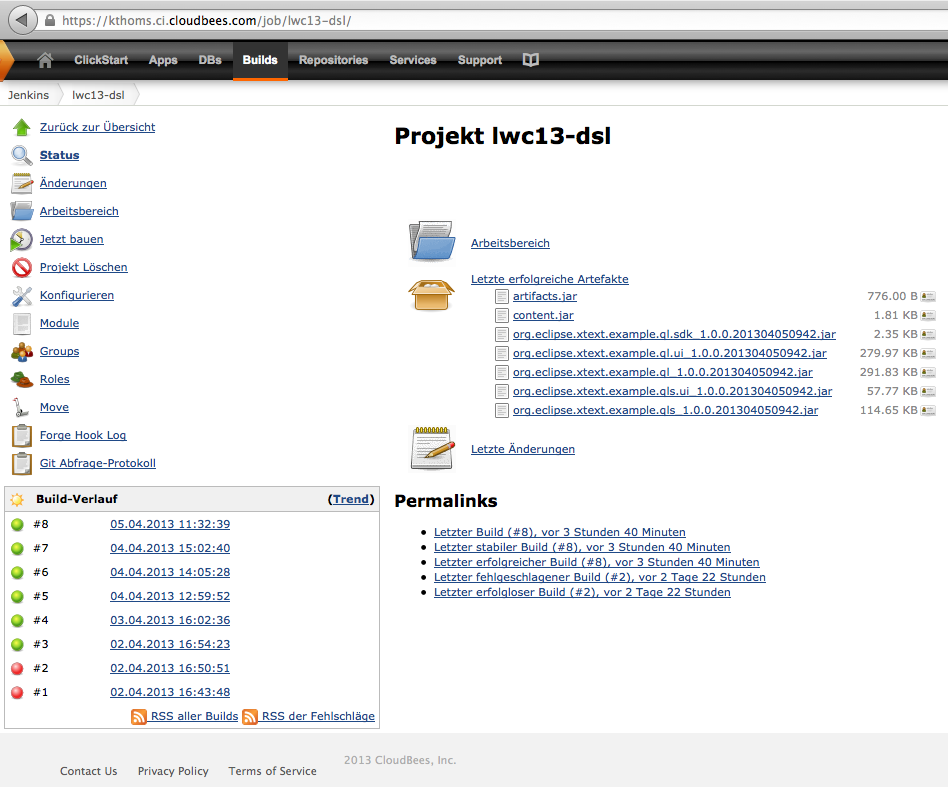
\includegraphics[width=15cm]{images/chapter04/jenkins-1.png}

This build could be reproduced on any Jenkins server with the following
configuration settings:
\begin{itemize}
  \item Create a job of style ``Maven2/3''
  \item Git repository URL:\newline
  \texttt{https://code.google.com/a/eclipselabs.org/p/lwc13-xtext/}
  \item Build-trigger: poll repository every 30 minutes
\begin{lstlisting}
*/30 * * * *
\end{lstlisting}
  \item In the Maven build section, choose a Maven 3 installation
  \item Configure POM: \texttt{projects/pom.xml}
  \item Goals and options: \texttt{clean install}
  \item Alternative settings file (Advanced options): \texttt{devenv/lwc13.devenv/settings.xml}
  \item Add post-build action - archive artifacts:
  \texttt{projects/*/target/repository/**}
\end{itemize}

